\documentclass[handout]{beamer}
\usepackage[utf8]{inputenc}
\usepackage{amsmath, pdfpages, pdflscape, lscape, color, listings, hyperref, amssymb, graphicx,textcomp,varioref, afterpage, subcaption, float, bm, tikz} 


\newcommand{\Fig}[1]{Figure \ref{#1}}
\newcommand{\fig}[1]{figure \ref{#1}}
\newcommand{\tab}[1]{table \ref{#1}}
\newcommand{\eq}[1]{equation \ref{#1}}
\newcommand{\Eq}[1]{Equation \ref{#1}}
\newcommand{\alg}[1]{algorithm \ref{#1}}
\newcommand{\Alg}[1]{Algorithm \ref{#1}}
\newcommand{\chp}[1]{chapter  \ref{#1}}
\newcommand{\Chp}[1]{Chapter  \ref{#1}}
\newcommand{\e}[1]{\cdot 10^{#1}}
\newcommand{\h}{\hbar}
\newcommand{\der}[2]{\frac{\partial #1}{\partial #2}}
\newcommand{\dder}[2]{\frac{\partial^2 #1}{\partial #2^2}}
\newcommand{\p}{\boldsymbol{P}}
\newcommand{\q}{\boldsymbol{q}}
\newcommand{\norm}[1]{\left\lVert#1\right\rVert}
\newcommand{\coef}[2]{\frac{\langle #1,#2\rangle_Q}{\norm{#2}^}}


\newenvironment{test}[1]
{
 \usebackgroundtemplate{}
 \color{gray!30!black}
   \begin{tikzpicture}[remember picture, overlay]
     \node[anchor = center, opacity=.25] (image) at (current page.center) {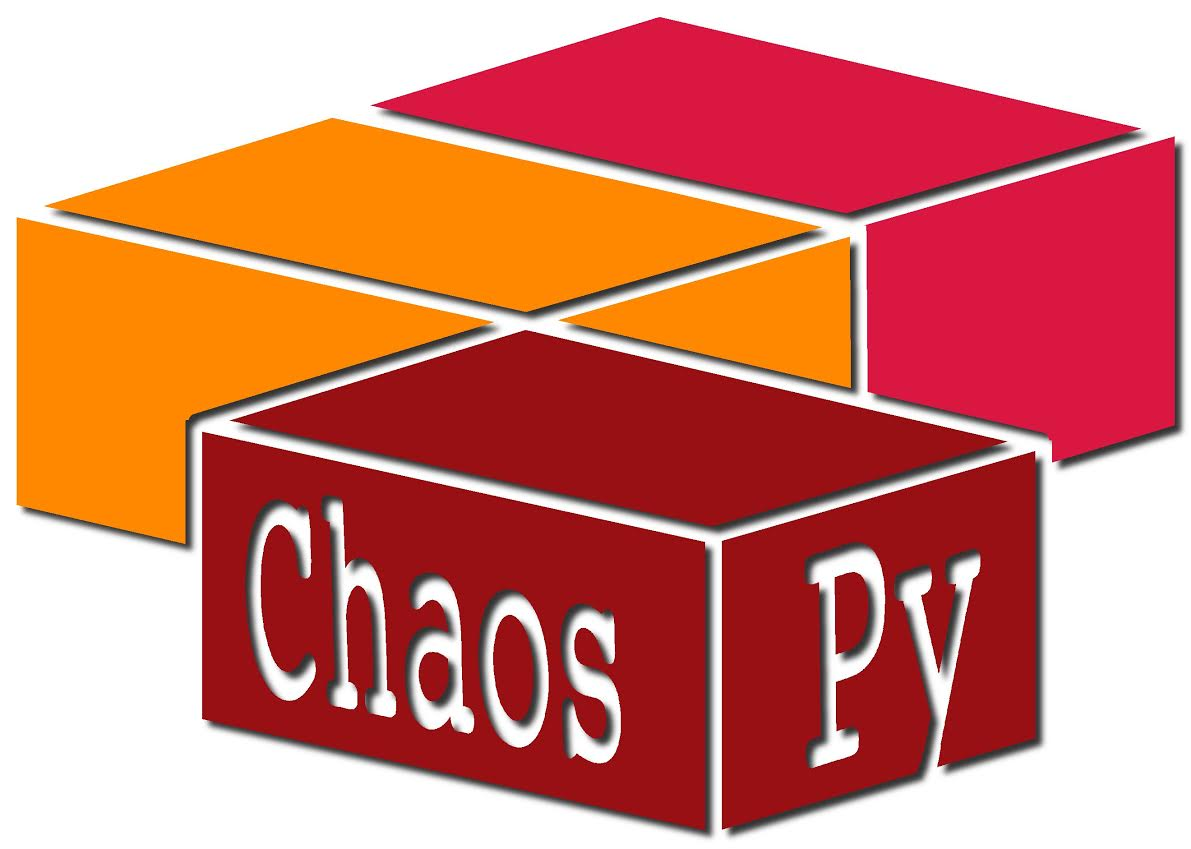
\includegraphics[scale=0.25]{chaospy_logo.jpg}};
   \end{tikzpicture}
 \begin{frame}[fragile,enviroment=chaospy]
   
}
{
 \end{frame}
}


\newenvironment{chaospy}[1]
{\color{gray!30!black}
     \color{gray!30!black}
     \usebackgroundtemplate{
   \begin{tikzpicture}[remember picture, overlay]
     \node[anchor = center, opacity=.25] (image) at (current page.center) {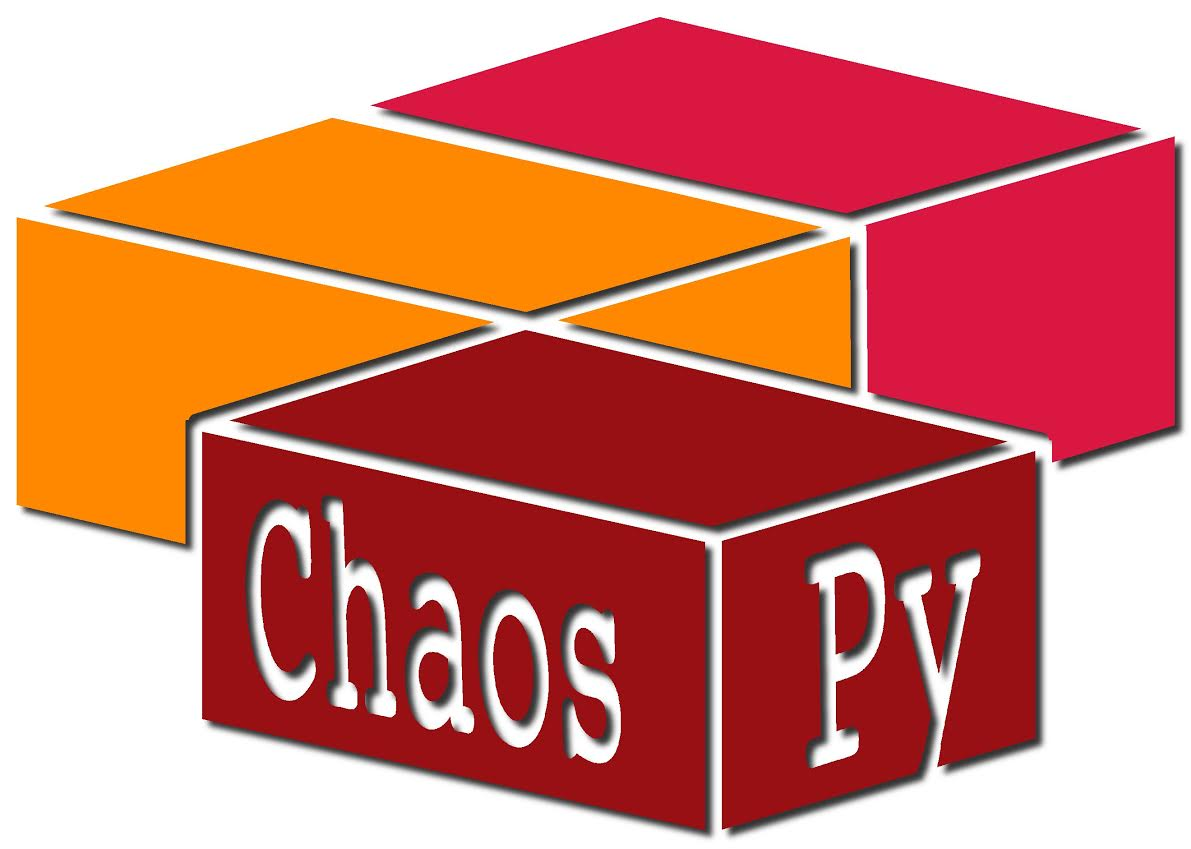
\includegraphics[scale=0.25]{chaospy_logo.jpg}};
   \end{tikzpicture}}
     \begin{frame}[fragile,environment=chaospy]
    \frametitle{{#1}}}
{\end{frame}}


\definecolor{keywords}{RGB}{255,0,90}
\definecolor{comments}{RGB}{0,0,113}
\definecolor{red}{RGB}{160,0,0}
\definecolor{green}{RGB}{0,150,0}
 
\usetheme{kalkulo}

\graphicspath{{./figures/}}


\title{Polynomial chaos expansions part I: Method Introduction}
\author{Jonathan Feinberg and Simen Tennøe}


\begin{document}



\begin{frame}
  \maketitle
\end{frame}


\begin{chaospy}{Introduction to Chaospy}
  Chaospy is a Python toolbox specifically developed by yours truly to implement polynomial chaos expansions.\newline
  
  \pause
  \begin{alert}{Task: Install Chaospy by following the instructions}\newline
    
    \href{https://github.com/hplgit/chaospy}{https://github.com/hplgit/chaospy}
    %\newline \href{https://github.com/hplgit/chaospy}{\beamergotobutton{Chaospy}}
  \end{alert}
\end{chaospy}


\section{Introduction}
\begin{frame}
  \frametitle{Introducing the problem}
  We have a simple differential equation
  \begin{align*}
    \frac{d u(x)}{dx} & =-au(x),\qquad u(0) = I,
  \end{align*}
  where $a$ and $I$ are uncertain.\newline
  
  \pause
  Standard notation
  \begin{itemize}
    \item $u(\mathbf{x}, \mathbf{q})$ - Solution to the differential equation.
    \item $\mathbf{q}$ - Parameters with uncertanties, $a$ and $I$.
    \item $D$ - The number of input parameters, $D=2$.
  \end{itemize}
\end{frame}

\begin{frame}
  \frametitle{Probability space}
  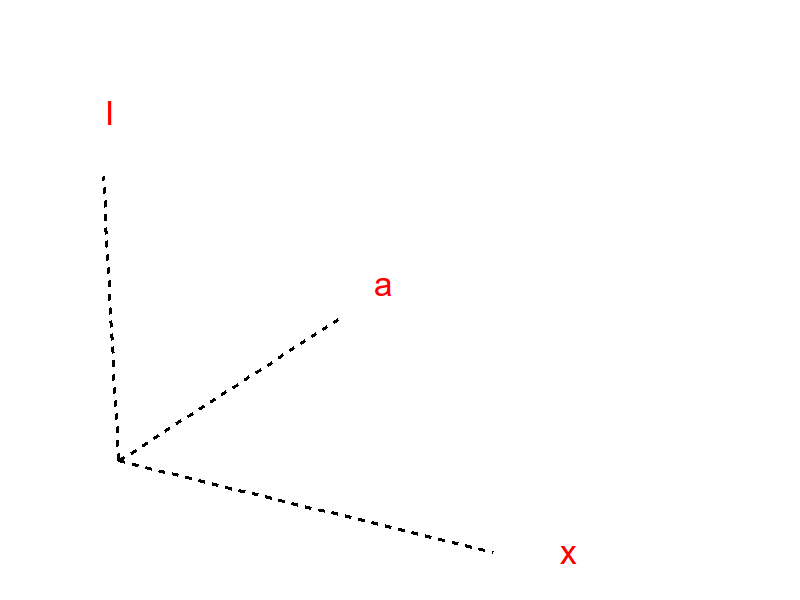
\includegraphics[width=\textwidth]{probspace.png}
\end{frame}







\subsection{Monte Carlo Sampling}

\begin{frame}[fragile]
  \frametitle{One traditional way to solve this problem has been to use Monte Carlo sampling.}
    \begin{figure}
    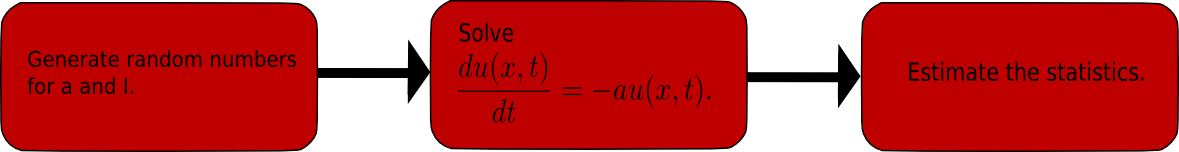
\includegraphics[width=\textwidth]{MC.png}
  \end{figure}
\begin{lstlisting}[language=python]
  import chaospy as cp
  import numpy as np

  def u(x, a, I):
    return I*np.exp(-a*x)
    
  N = 1000

  a = cp.Uniform()
  I = cp.Uniform()

  samplesI = I.sample(N)
  samplesa = a.sample(N)
  x = np.linspace(0, 10, N)

  U = u(x, samplesa, samplesI)

  E = np.sum(U)/N
  Var = np.sum(U**2)/N - E**2

  print "E = ", E
  print "Var = ", Var
\end{lstlisting}

    
\end{frame}


\begin{frame}
  \frametitle{Convergence of Monte Carlo Sampling}

  \begin{figure}
    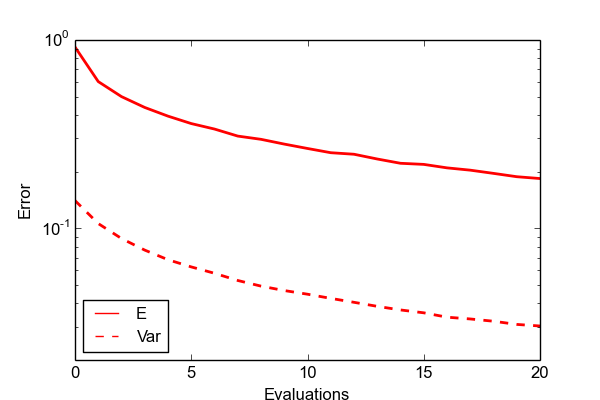
\includegraphics[width=0.8\textwidth]{MC_convergence_1D_1.png}
  \end{figure}
  
\end{frame}



\section{Polynomial Chaos}


\begin{frame}
  \frametitle{The general idea behind polynomial chaos expansion}
   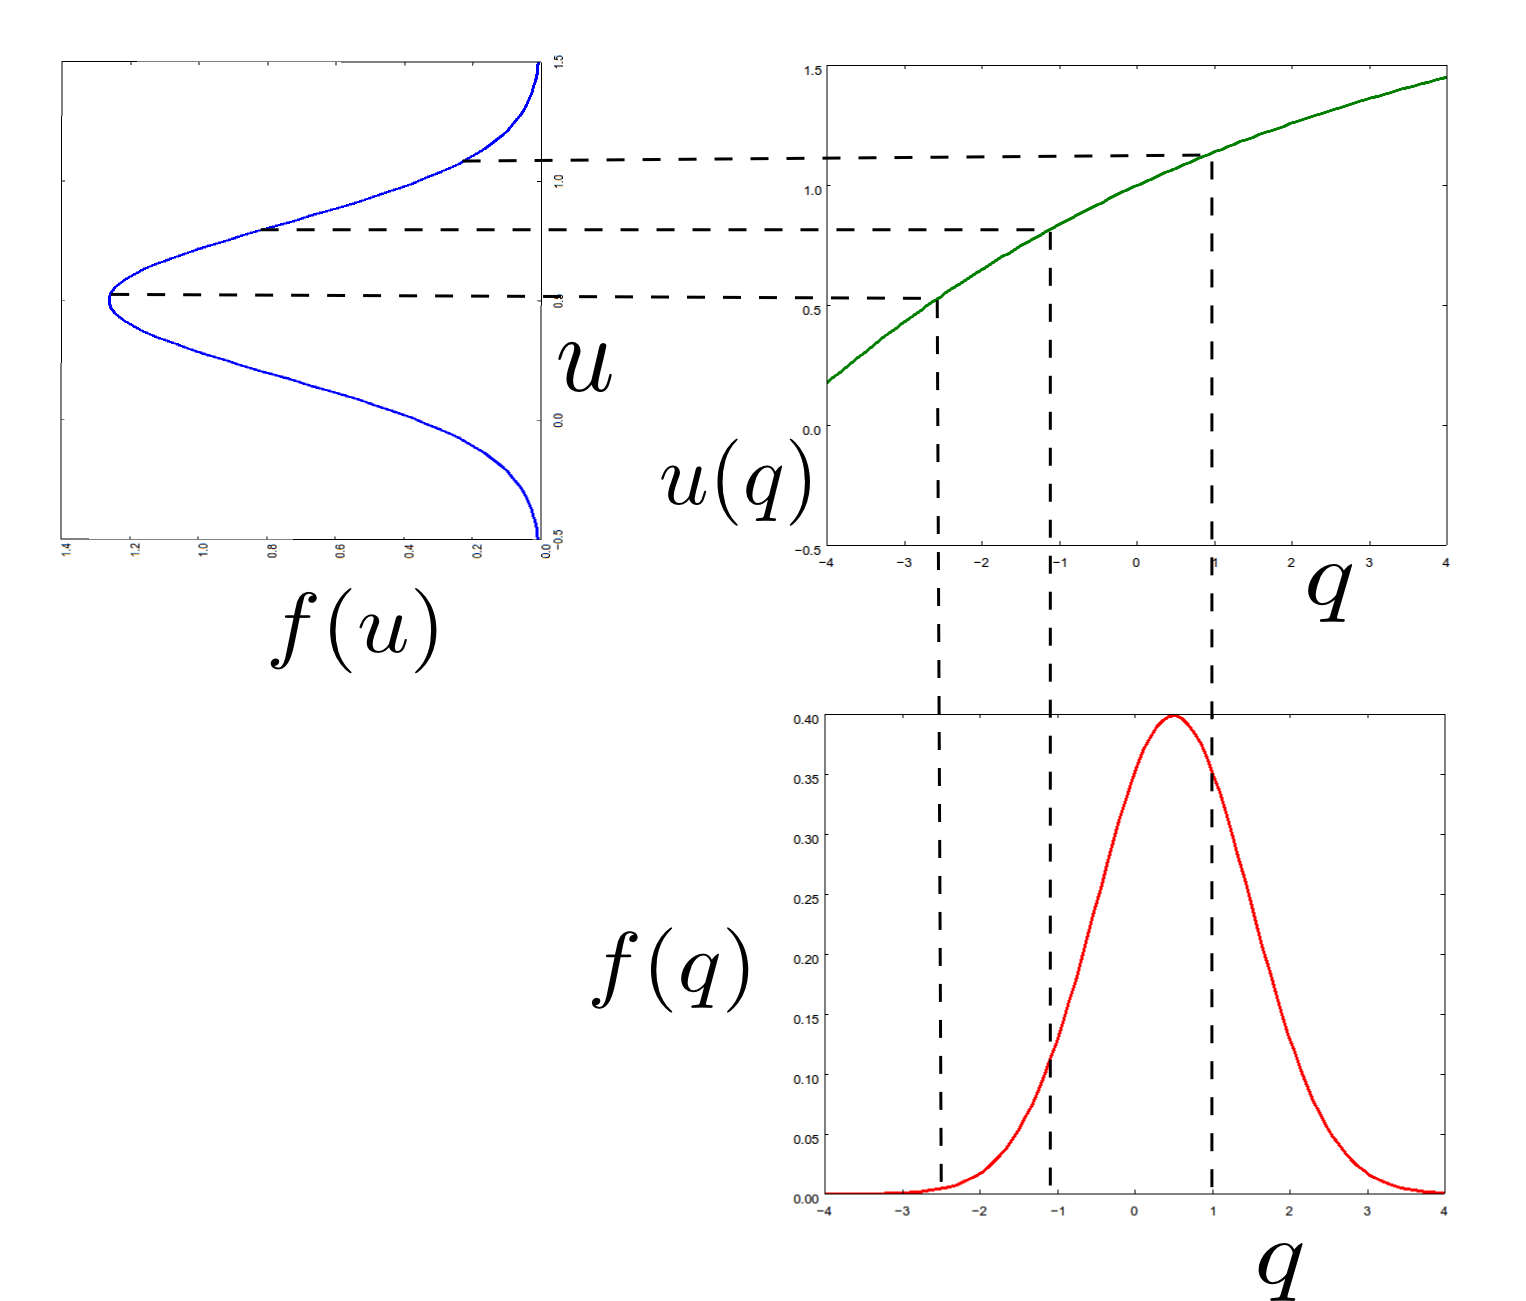
\includegraphics[width=0.8\textwidth]{mapping.png}
\end{frame}



\begin{frame}
  \frametitle{Construct polynomial approximation}
  \begin{columns}[c] 
    \column{.5\textwidth}
      Multi-index\\
    \begin{tabular}{c}
    \\
      $\mathbf{P}_{00}$\\
    $\mathbf{P}_{10} \quad \mathbf{P}_{01}$\\
    $\mathbf{P}_{20} \quad \mathbf{P}_{11}\quad \mathbf{P}_{02}$\\
    $\mathbf{P}_{30} \quad \mathbf{P}_{21}\quad \mathbf{P}_{12}\quad ...$ 
  \end{tabular}

\column{.5\textwidth}

Single-index\\
\begin{tabular}{c}
\\
    $\mathbf{P}_{0}$\\
    $\mathbf{P}_{1} \quad \mathbf{P}_{2}$\\
    $\mathbf{P}_{3} \quad \mathbf{P}_{4}\quad \mathbf{P}_{5}$\\
    $\mathbf{P}_{6} \quad \mathbf{P}_{7}\quad \mathbf{P}_{8}\quad ...$ 
  \end{tabular}
  \end{columns}
\end{frame}

\begin{frame}
  \frametitle{Convergence of polynomial approximation}

  \begin{figure}
    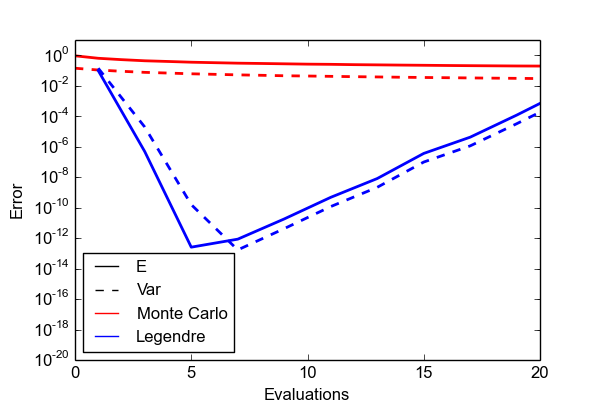
\includegraphics[width=0.8\textwidth]{MC_convergence_1D_2.png}
  \end{figure}
  
\end{frame}


\begin{frame}
  \frametitle{Inner product and orthogonality}

    \begin{align*}
    \langle U,V \rangle &= E(V\cdot V)\\
    \pause
    &= \int f_Q(q)U(x,q)V(x,q)dq
  \end{align*}

  \pause
  Orthogonality
  \[\langle P_n,P_m\rangle =
  \begin{cases}
    \norm{P_n}^2_Q & n = m \\
    0 & n \neq M
  \end{cases}\]

\end{frame}

\begin{frame}
\frametitle{Why is this a good idea?}
\begin{block}{Theorem}
  \[\norm{U-\hat{U}_m}_Q \leq \norm{U-U^*}_Q \qquad \text{for all } U^* \in \mathbb{P}_M\]
\end{block}
Assumptions: 
\begin{itemize}
  \item $P_0,...,P_N$ are mutually orthogonal
  \item $c_0,...,c_N$ are Fourier coefficients, $c_n = \frac{\langle U, P_n\rangle}{\norm{P_n}^2_Q}$
 \end{itemize}
 This also leads to 
  \[\text{Var}(|U-\hat{U}_m|)\leq \text{Var}(|U-U^*|)_Q \qquad \text{for all } U^* \in \mathbb{P}_M\]
\end{frame}

\begin{frame}
 \frametitle{When we have constructed $\hat U_M$ we also know}
   \begin{align*}
  \mathbb E[\hat u_M] &= c_0\\
  \mathbb V[\hat u_M] &= \sum_{n=1}^N c_i^2\norm{\p_n}_{Q}^2
  \end{align*}
\end{frame}

\begin{frame}
 \frametitle{This leaves us with the following two challenges}
 
 Finding
 \begin{itemize}
  \item $P_0,...,P_N$
  \item $c_0,...,c_N$
 \end{itemize}

\end{frame}

\begin{frame}
 \frametitle{Proposal, let us use Gram-Schmidt to find the orthogonal polynomials}
 Assumption: We are in 1D and have $a ~ F_q$ and $I = 1$. 
 \[V_0, V_1,...,V_N = 1, q,...,q^N\]
 The Gram Schmidt method is
 
 \begin{align*}
    P_0 &= V_0\\
    P_n &= V_n - \sum_{m=0}^n \frac{\langle V_n,P_m\rangle_Q}{\norm{P_m}^2_Q}\\
  &= V_n - \sum_{m=0}^n\frac{\mathbb{E}(V_nP_m)}{\mathbb{E}(P_m^2)}
 \end{align*}

\end{frame}

\begin{chaospy}{Gram-Schmidt with chaospy}
\begin{lstlisting}[language=python]
M = 5; D = 1
N = factorial(M+D)/factorial(M) - 1
a = cp.Uniform()

V = cp.basis(0,M,1)
P_M =  [V[0]]

for n in xrange(1,N):
    summation = 0
    for m in xrange(0,n):
        summation += P_M[m]*cp.E(V[n]*P_M[m],a)
                            /cp.E(P_M[m]**2,a)
    P_M.append(V[n] - summation)
 \end{lstlisting}
\end{chaospy}


\begin{frame}
 \frametitle{Plot of all generated polynomials}
  \begin{figure}
    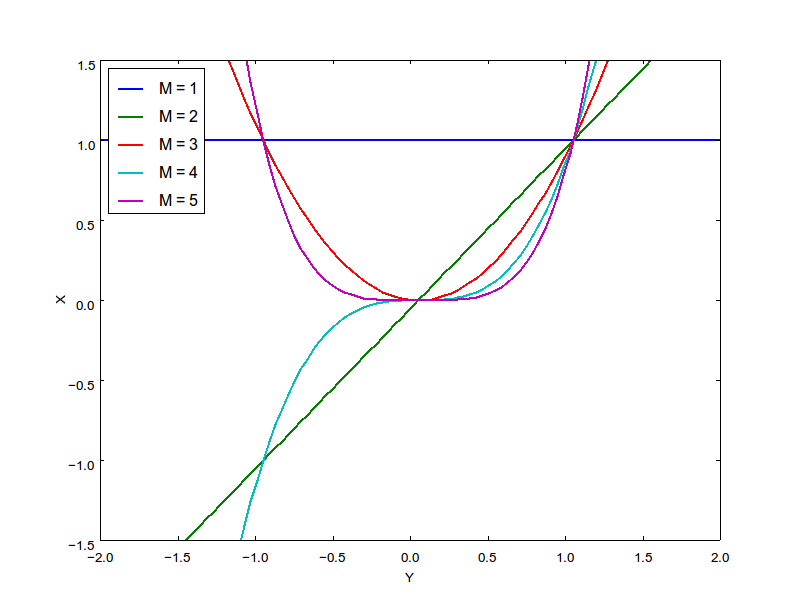
\includegraphics[width=0.8\textwidth]{gramschmidtpoly.png}
  \end{figure}
\end{frame}


\begin{frame}
 \frametitle{But once again things go wrong}
  %plot the errors as we go to large M
  
  
 \end{frame}


\begin{frame}
 \frametitle{The Three Term Recurrence (TTR) relation}
  All orthogonal polyomials satisfy the three term recurrence relation
  \[P_{N+1} = (x-A_n)P_n - B_nP_{n-1}\]
  \[P_{-1} = 0\qquad P_0 =1\]
    \pause
  
  \[A_n = \frac{\langle q,P_n\rangle_Q}{\norm{P_n}}\]
  \[B_n = 
  \begin{cases}
  \frac{\norm{P_n}^2_Q}{\norm{P_{n-1}}} \qquad n > 0\\
  \norm{P_n}^2_Q \qquad n = 0
  \end{cases}
  \]
  \end{frame}

\begin{chaospy}{TTR with chaospy}
\begin{lstlisting}[language = Python]
import chaospy as cp

M = 3
a = cp.Normal()
P = cp.orth_ttr(M, a)

print P
>>> [1.0, q0, q0^2-1.0, q0^3-3.0q0]
\end{lstlisting}
\end{chaospy}

  
  
\begin{frame}
 \frametitle{The Three Term Recurrence (TTR) relation}
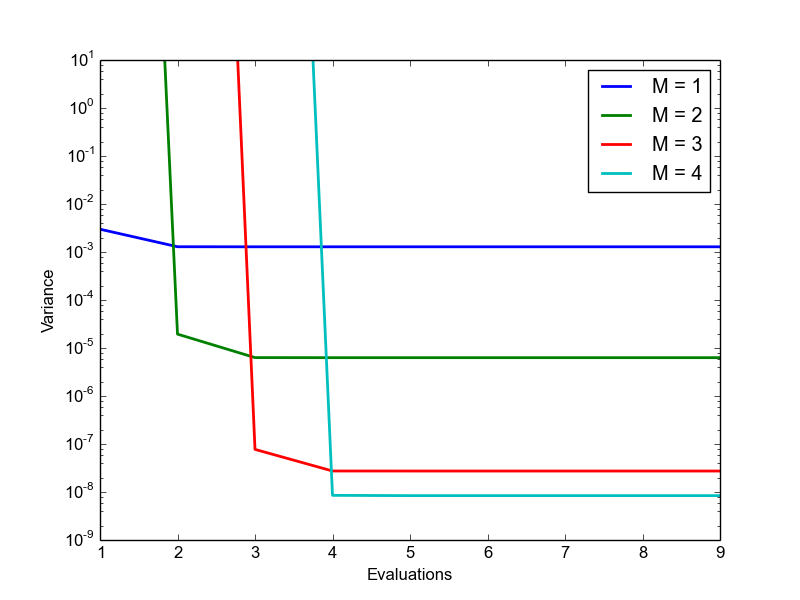
\includegraphics[width=0.9\textwidth]{k_convergence.png}
 \end{frame}


\begin{chaospy}{Finding the Fourier coefficients}
 \begin{lstlisting}[language=python]
a = cp.Uniform(0,0.1)

def u(x,a):
  ax = np.outer(a,x)
  return np.exp(-ax)

m = 2
x = np.linspace(0, 10, 100)

P, norm = cp.orth_ttr(m, a, retall=True)
nodes, weights = cp.generate_quadrature(m+1, a,
                                        rule="G")
solves = u(x,nodes[0])
U_hat, c = cp.fit_quadrature(P, nodes, weights,
                             solves,retall=True)
\end{lstlisting}

\end{chaospy}


\begin{frame}
\frametitle{Convergence of orthogonal polynomial approximation}

  \begin{figure}
    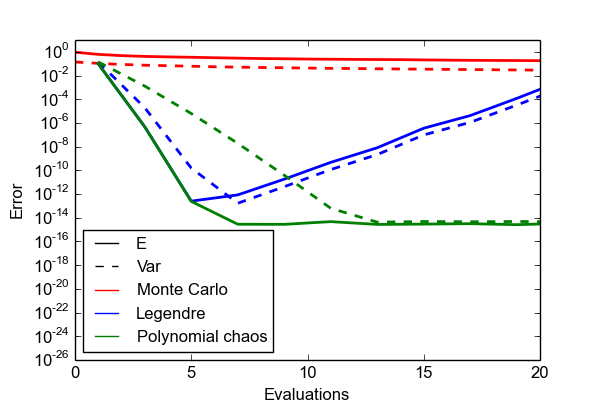
\includegraphics[width=0.8\textwidth]{MC_convergence_1D_3.png}
  \end{figure}
   \end{frame}


\begin{frame}
 \frametitle{Multidimensional problems}
  \begin{align*}
  P_n &= P^{(1)}_n, ..., P^{(D)}_{n_D}
  & n\longleftrightarrow (n_1, ..., n_D)
  \end{align*}
  \pause
  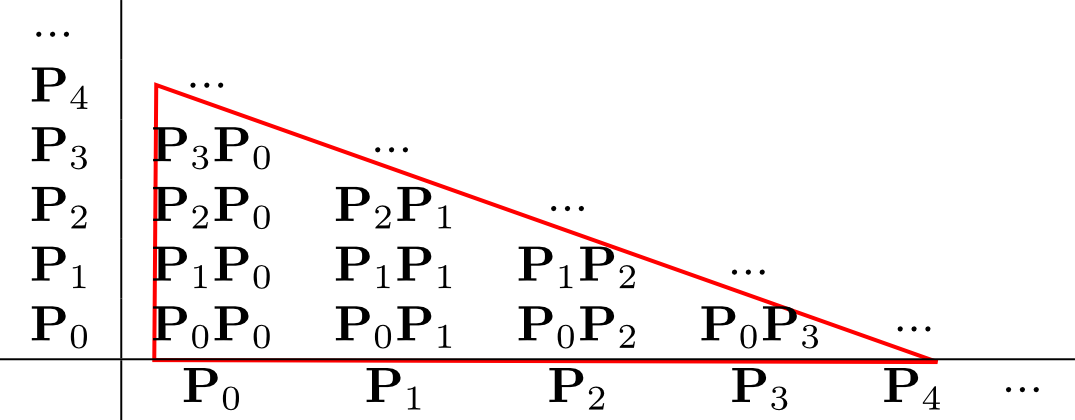
\includegraphics[width=\textwidth]{multidim.png}
   
 % \begin{tabular}{l|cccccc}
 % ... &&&&&\\ 
  % $\mathbf{P}_{4}$& ...&&&& \\
 %   $\mathbf{P}_{3}$ &	$\mathbf{P}_{3}\mathbf{P}_{0}$ & ... && &\\
 %   $\mathbf{P}_{2}$ &	$\mathbf{P}_{2}\mathbf{P}_{0}$ & $\mathbf{P}_{2}\mathbf{P}_{1}$ & ... &&& \\
 %   $\mathbf{P}_{1}$ &	$\mathbf{P}_{1}\mathbf{P}_{0}$ &$\mathbf{P}_{1}\mathbf{P}_{1}$& $\mathbf{P}_{1}\mathbf{P}_{2}$ & ...&&\\
 %   $\mathbf{P}_{0}$ &	$\mathbf{P}_{0}\mathbf{P}_{0}$ &$\mathbf{P}_{0}\mathbf{P}_{1}$& $\mathbf{P}_{0}\mathbf{P}_{2}$ & $\mathbf{P}_{0}\mathbf{P}_{3}$ & ...\\ \hline
%		     &	$\mathbf{P}_{0}$	&$\mathbf{P}_{1}$& $\mathbf{P}_{2}$ & $\mathbf{P}_{3}$ & $\mathbf{P}_{4}$& ...
%  \end{tabular}
 \end{frame}


\begin{frame}
 \frametitle{Multidimensional orthogonality}
\begin{align*}
 \langle P_n, P_m\rangle &= \mathbb{E}(P_{n_1}^{(1)}\cdots P_{n_D}^{(D)}\cdot P_{m_1}^{(1)}\cdots P_{m_D}^{(D)}\\
  &= \mathbb{E}(P_{n_1}^{(1)}\cdot P_{m_1}^{(1)})\cdots \mathbb{E}(P_{n_D}^{(D)}\cdot P_{m_D}^{(D)}) \\
  &= \langle P_{n_1}^{(1)}\cdot P_{m_1}^{(1)} \rangle\cdots  \langle P_{n_D}^{(D)}\cdot P_{m_D}^{(D)} \rangle \\
  &= \begin{cases}
       0 & n_d \neq m_d \quad \text{There exists a } d \text{ such that }n \neq m\\
      \norm{P}^2 & \text{else} 
     \end{cases}
\end{align*}

 \end{frame}


 
 \begin{chaospy}{Code example}
\begin{lstlisting}[language = Python]
import chaospy as cp
I = cp.Uniform()
a = cp.Normal()
dist = cp.J(a,I)

P = cp.orth_ttr(1, dist)
print P
>>> [1.0, q1-0.5, q0]

P = cp.orth_ttr(3, dist)
print cp.E(P[1]*P[2],dist)
>>> 0.0
print cp.E(P[3]*P[3],dist)
>>> 0.00555555555556

\end{lstlisting}
\end{chaospy}
 
 
 \begin{chaospy}{Convergence of multdimensional problem}
 \begin{lstlisting}[language=python]
def u(x,a, I):
  return I*np.exp(-a*x)
 
a = cp.Uniform(0, 0.1); I = cp.Uniform(8, 10)
dist = cp.J(a,I)
x = np.linspace(0, 10, 100)
m = 2

P = cp.orth_ttr(m, dist)
nodes, weights = cp.generate_quadrature(m+1, dist,
                                        rule="G")
i1,i2 = np.mgrid[:len(weights), :100]
solves = u(x[i2],nodes[0][i1],nodes[1][i1])
U_hat = cp.fit_quadrature(P, nodes, weights,
                          solves)
 \end{lstlisting}
\end{chaospy}

 
\begin{frame}
 \frametitle{Convergence}
\begin{figure}
    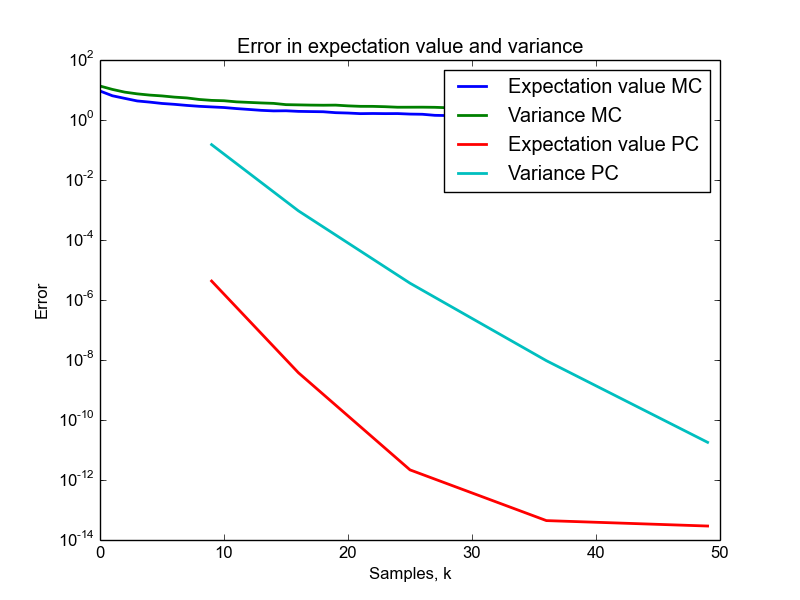
\includegraphics[width=0.8\textwidth]{MC_convergence_2D.png}
  \end{figure}

 \end{frame}
 
 
 
 
 
 
 

\begin{frame}
  \frametitle{The curse of dimensionality}
  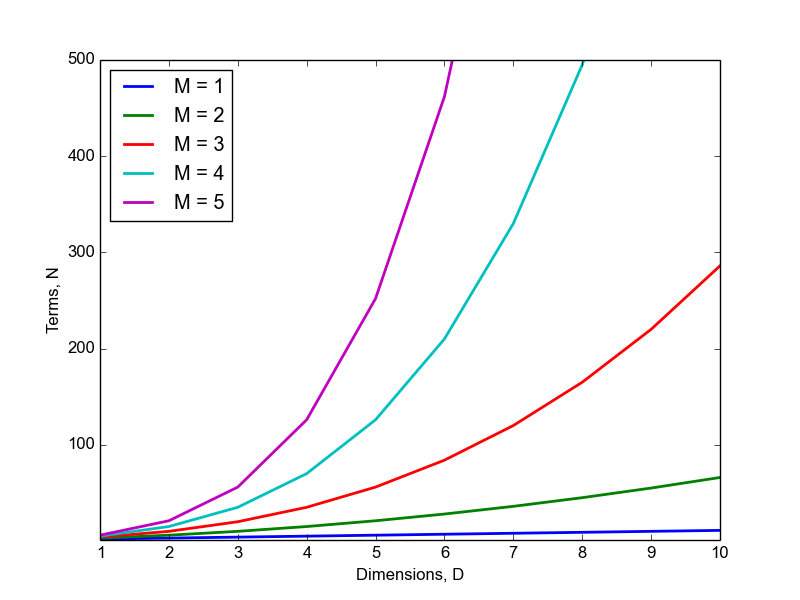
\includegraphics[height = 0.9\textheight]{dimensionality.png}

\end{frame}


\begin{frame}
  \frametitle{Gibb's Phenomena, discontinues methods are troublesome}
  \begin{figure}
  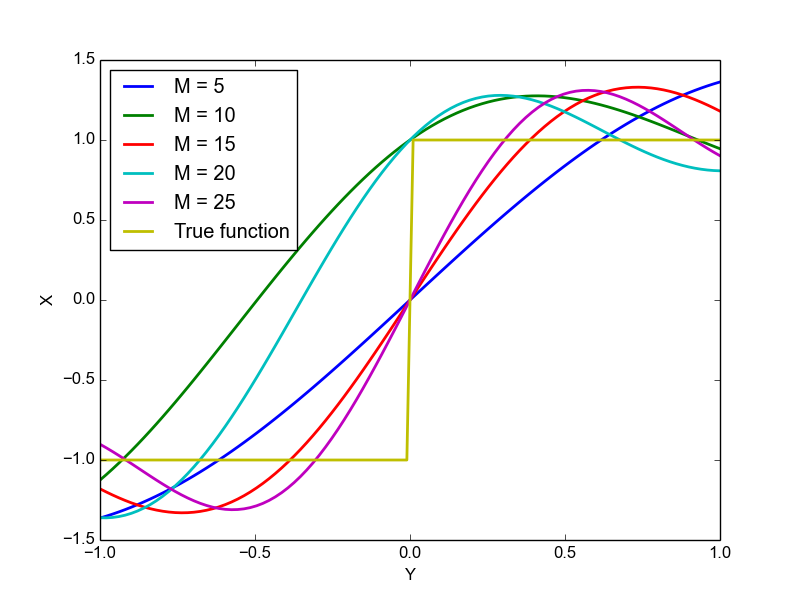
\includegraphics[width=0.8\textwidth]{gibbs.png}
  \end{figure}

  \end{frame}















 

\if f
%\begin{frame}
%  \frametitle{What happens if we choose the wrong distribution}
  
%\end{frame}



\begin{frame}
  \frametitle{Polynomial Chaos}
  In polynomial chaos expansion we approximates the solution $u$ with $\hat u$ by using orthogonal polynomials.
  \[\hat u_m = \sum_{i=0}^N c_i \p_i\]
  where N is given by the order of the expansion, M, as
  \[N + 1 =\frac{(M + D)!}{M!D!}\]
\end{frame}


\begin{frame}
  \frametitle{Polynomial Chaos}
  The general idea behind Polynomial Chaos expansion is
  \[E[\p_m(Z)\p_n(Z)] = \sum_i \p_m(z_i)_n(z_i)\rho_i\]
\end{frame}



\begin{frame}
  \frametitle{Orthogonal polynomials, $\p$}
  Because the orthogonal polynomials depend on the density function $p_\xi$, they must be chosen differently for each random variable.\newline

  They can be calculated using the three-term recurence (TTR) formula.\newline

\end{frame}


\begin{frame}
  \frametitle{Fourier Coefficients, $c_i$}
  Defined as
  \[c_i = \frac{\langle u,\p_i\rangle_{\q}}{\norm{\p_i}_{\q}}\]
  Most often found numericaly by either
  \begin{itemize}
    \item Galerkin method
    \item Colocation method
  \end{itemize}
\end{frame}


\begin{frame}
  \frametitle{The polynomial is assembled and the goal is}
  \begin{align*}
  \mathbb E[\hat u_M] &= c_0\\
  \mathbb V[\hat u_M] &= \sum_{i=1}^N c_i^2\norm{\p_i}_{\q}^2
  \end{align*}
\end{frame}







\begin{chaospy}{Simple example using Chaospy}
  Problem:
  \[\frac{d u(x,t)}{dt} =-au(x,t),\qquad u(x, 0) = I(x)\]
  $I(x)$ is precicly know, while $a$ is uncertain, with a uniform distribution.\newline

  Find the expectation value, $\mathbb E$, and and the variance $\mathbb V$.
  

\end{chaospy}




\begin{frame}
  \frametitle{Standard notation}
  \begin{itemize}[<+->]
     \item $c_i(\mathbf{x})$ - Polynomial coefficients, shorthand $c_i$.
    \item $\mathbf{P}_i(\mathbf{q})$ - Orthogonal polynomials, shorthand $\mathbf{P}_i$.
  \end{itemize}
\end{frame}
\fi

\end{document}
